%!TEX root=../sbc-template.tex

\chapter{Resultados e Discussão} \label{cap:resultados}

Para a execução dos \emph{scripts} de treinamento foi utilizado um servidor com a seguinte configuração: processador Intel(R) Core(TM) i7-8700 CPU @ 3.20GHz, $32$ GB de memória principal, $960$ GB de memória secundária e $2$ placas de vídeo NVIDIA GTX 1080 Ti com $11$ GB de VRAM para aceleração em \emph{hardware} do treinamento. Os resultados obtidos da aferição do desempenho para as diferentes configurações propostas encontram-se dispostos na Tabela \ref{tab:resultadosExperimentais}.


\begin{table}[h!]
\caption{Síntese dos resultados experimentais.} \label{tab:resultadosExperimentais}
\begin{footnotesize}
\begin{tabular}{ccccccccc}
\toprule
\textbf{Modelo} & \textbf{Versão} &\textbf{Épocas} &\textbf{Precisão} & \textbf{Revocação} & \textbf{F-\emph{Score}} & \textbf{mAP@0.5} & \textbf{Parâmetros} & \textbf{Tempo}\\
\midrule
\textbf{YOLOv5} & \emph{Nano} &  $293/300$ & $\SI{79,5}{\percent}$ & $\SI{77,5}{\percent}$ & $\SI{78,48}{\percent}$ & $\SI{78,3}{\percent}$ & $\num{1760518}$ & $\SI{10}{\hour}\SI{19}{\minute}$\\
\textbf{YOLOv5} & \emph{Small} & $173/300$ & $\SI{81,5}{\percent}$ & $\SI{79,7}{\percent}$ & $\SI{80,58}{\percent}$ & $\SI{80,7}{\percent}$ & $\num{7012822}$ & $\SI{7}{\hour}\SI{26}{\minute}$\\
\textbf{YOLOv5} & \emph{Medium} & $300/300$ & $\SI{59,5}{\percent}$ & $\SI{63,1}{\percent}$ & $\SI{61,20}{\percent}$ & $\SI{55,5}{\percent}$ & $\num{20852934}$ & $\SI{9}{\hour}\SI{7}{\minute}$\\
\midrule
\textbf{YOLOv5} & \emph{Nano} &  $500/500$ & $\SI{79,9}{\percent}$ & $\SI{78,2}{\percent}$ & $\SI{79,04}{\percent}$ & $\SI{79,0}{\percent}$ & $\num{1760518}$ & $\SI{12}{\hour}\SI{38}{\minute}$\\
\textbf{YOLOv5} &\emph{Small} &  $194/500$ & $\SI{81,4}{\percent}$ & $\SI{79,4}{\percent}$ & $\SI{80,38}{\percent}$ & $\SI{80,4}{\percent}$ & $\num{7012822}$ & $\SI{6}{\hour}$\\
\textbf{YOLOv5} & \emph{Medium} & $264/500$ & $\SI{81,7}{\percent}$ & $\SI{78,9}{\percent}$ & $\SI{80,27}{\percent}$ & $\SI{79,9}{\percent}$ & $\num{20852934}$ & $\SI{9}{\hour}\SI{58}{\minute}$\\
\midrule
\textbf{YOLOv7} &  \emph{Tiny} & $500/500$ & $\SI{75,2}{\percent}$ & $\SI{77,9}{\percent}$ & $\SI{76,52}{\percent}$ & $\SI{77,0}{\percent}$ & $\num{6007596}$ & $\SI{23}{\hour}\SI{1}{\minute}$\\
\textbf{YOLOv7}  & \emph{Normal} & $500/500$ & $\SI{79,2}{\percent}$ & $\SI{78,8}{\percent}$ & $\SI{78,99}{\percent}$ & $\SI{79,8}{\percent}$ & $\num{36481772}$ & $\SI{26}{\hour}\SI{34}{\minute}$\\
\textbf{YOLOv7} & \emph{X} & $500/500$ & $\SI{80,6}{\percent}$ & $\SI{79,9}{\percent}$ & $\SI{80,24}{\percent}$ & $\SI{81,4}{\percent}$ & $\num{70782444}$ & $\SI{52}{\hour}\SI{5}{\minute}$\\
\bottomrule
\end{tabular}
\end{footnotesize}
\end{table}

Ao tomar o F-\emph{Score} aferido em todos os experimentos, tem-se que a escolha de detectores de objetos baseados em \emph{Deep Learning} da Família YOLO mostrou-se uma escolha acertada, pois em $\SI{90}{\percent}$ dos cenários essa métrica mostrou-se acima de $\SI{78}{\percent}$. Ao tomar o mAP@0.5, uma métrica de referência no âmbito da detecção de objetos, verifica-se que esta também foi alta, sendo superior a $\SI{77}{\percent}$ no mesmo quantitativo de experimentos. Este argumento é corroborado pelo fato da Família YOLO ser estado da arte em diversas tarefas de detecção de objetos com \emph{Deep Learning} \cite{Sumit:YOLO}.

O modelo YOLOv5 \emph{Medium} obteve resultados contraintuitivos pois, quando treinado com $300$ épocas não incorreu em \emph{early stopping}, mas obteve o menor desempenho geral em termos de mAP@0.5. Esse resultado é indicativo de que uma grande quantidade de parâmetros não necessariamente implica em melhor desempenho. Apesar disso, no experimento em que foram consideradas $500$ épocas, visando favorecer um melhor ajuste de parâmetros, o modelo conseguiu melhor ajuste utilizando apenas $264$ épocas, com desempenho $\SI{30.53}{\percent}$ superior ao cenário anterior. Percebe-se, portanto, que o modelo em questão é de difícil ajuste fino e o seu desempenho é delicado em razão da flutuação estocástica, ou seja, não demonstra robustez.

O modelo YOLOv5 \emph{Nano} apresentou um bom desempenho no tocante ao mAP@0.5, embora tenha demandado mais tempo de treinamento dentre todos os YOLOv5 avaliados. Apesar disso,  esse é um dos modelos com maior potencial de uso prático em dispositivos embarcados, pois possui menor tempo de inferência dentre todos os avaliados em consequência do menor número de parâmetros.

Em relação aos modelos YOLOv7, as métricas obtidas foram parecidas com aquelas das YOLOv5, apesar de ser necessário ressaltar o aumento significativo no número de parâmetros, no tempo de treino e no número de épocas necessárias. Ressalta-se o modelo YOLOv7 \emph{X} como tendo obtido maior mAP@0.5 nos experimentos realizados. Os gráficos do monitoramento da perda e da acurácia desse modelo nos conjuntos de treinamento e validação encontram-se ilustrados na Figura \ref{fig:graph-train-val}. As Figuras \ref{ex:poucos} e \ref{ex:muitos} ilustram detecções de exemplos do conjunto de testes efetuadas por esse modelo, denotadas em azul, enquanto as caixas delimitadoras desejadas são denotadas em vermelho. É perceptível um bom grau de sobreposição entre os objetos desejados e os previstos pelo modelo, embora estes últimos venham a ter uma área menor que o esperado.


 \begin{figure}[h!]
 	\centering
 	\subfloat[Treinamento]{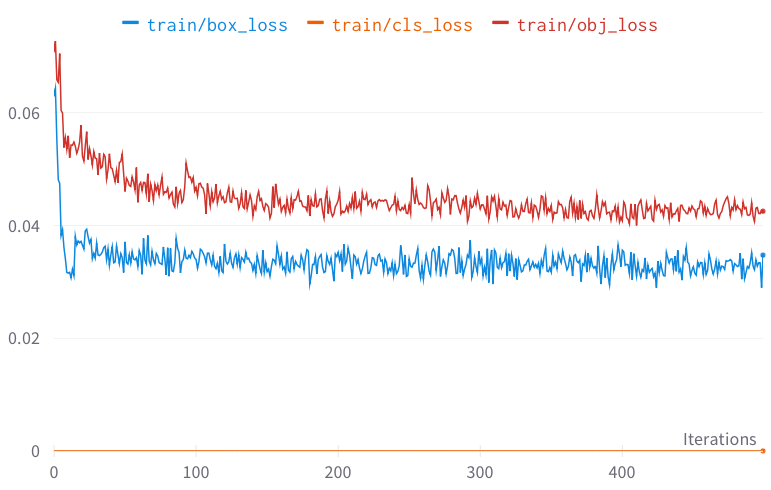
\includegraphics[width=0.8\linewidth]{./img/results/train.png}} \\
  \subfloat[Validação]{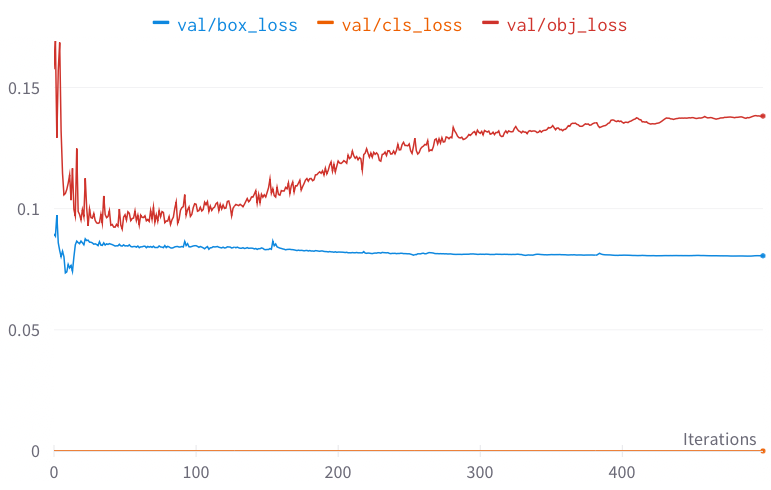
\includegraphics[width=0.8\linewidth]{./img/results/validation.png}}
 		\caption{Gráficos de monitoramento de métricas da YOLOv7 \emph{X} perante os conjuntos de treino e de validação.}  \label{fig:graph-train-val}
\end{figure}

 \begin{figure}[h!]
  	\centering
   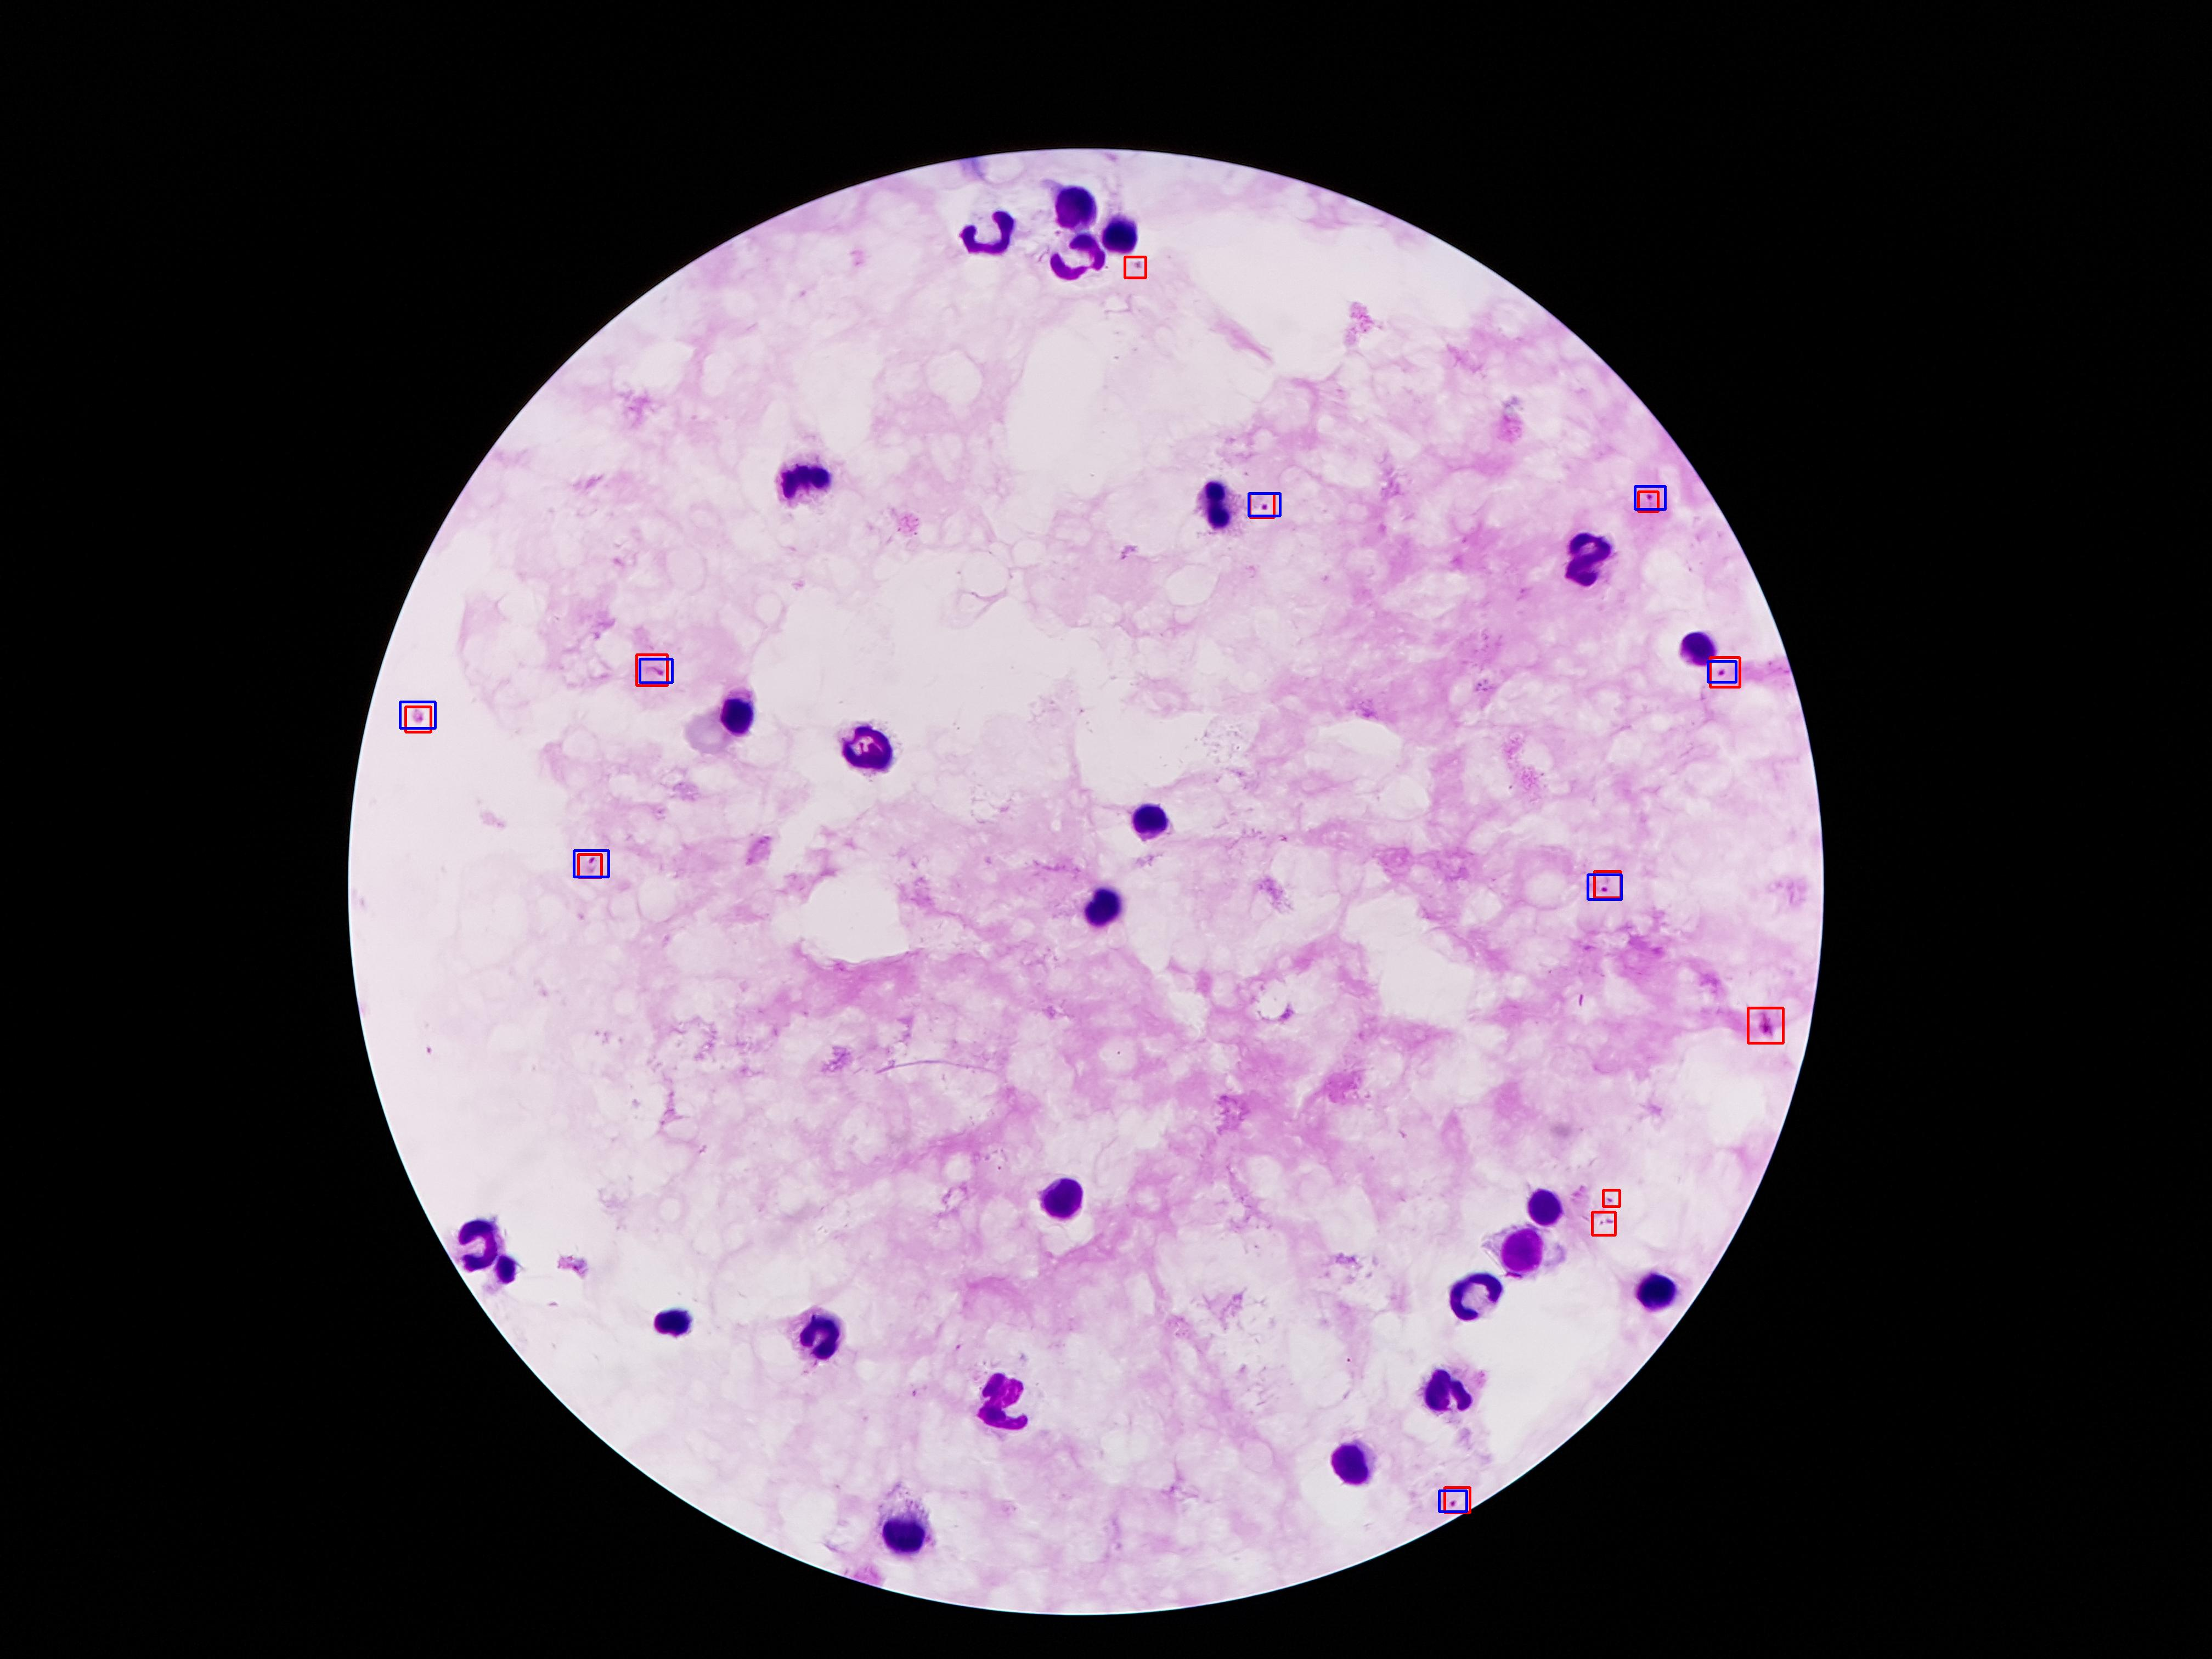
\includegraphics[width=\linewidth]{./img/full-predictions/result1-v7.jpg}
   \caption{Exemplo com poucos protozoários e suas respectivas detecções pela YOLOv7 \emph{X}.} \label{ex:poucos}
 \end{figure}

 \begin{figure}[h!]
  	\centering
   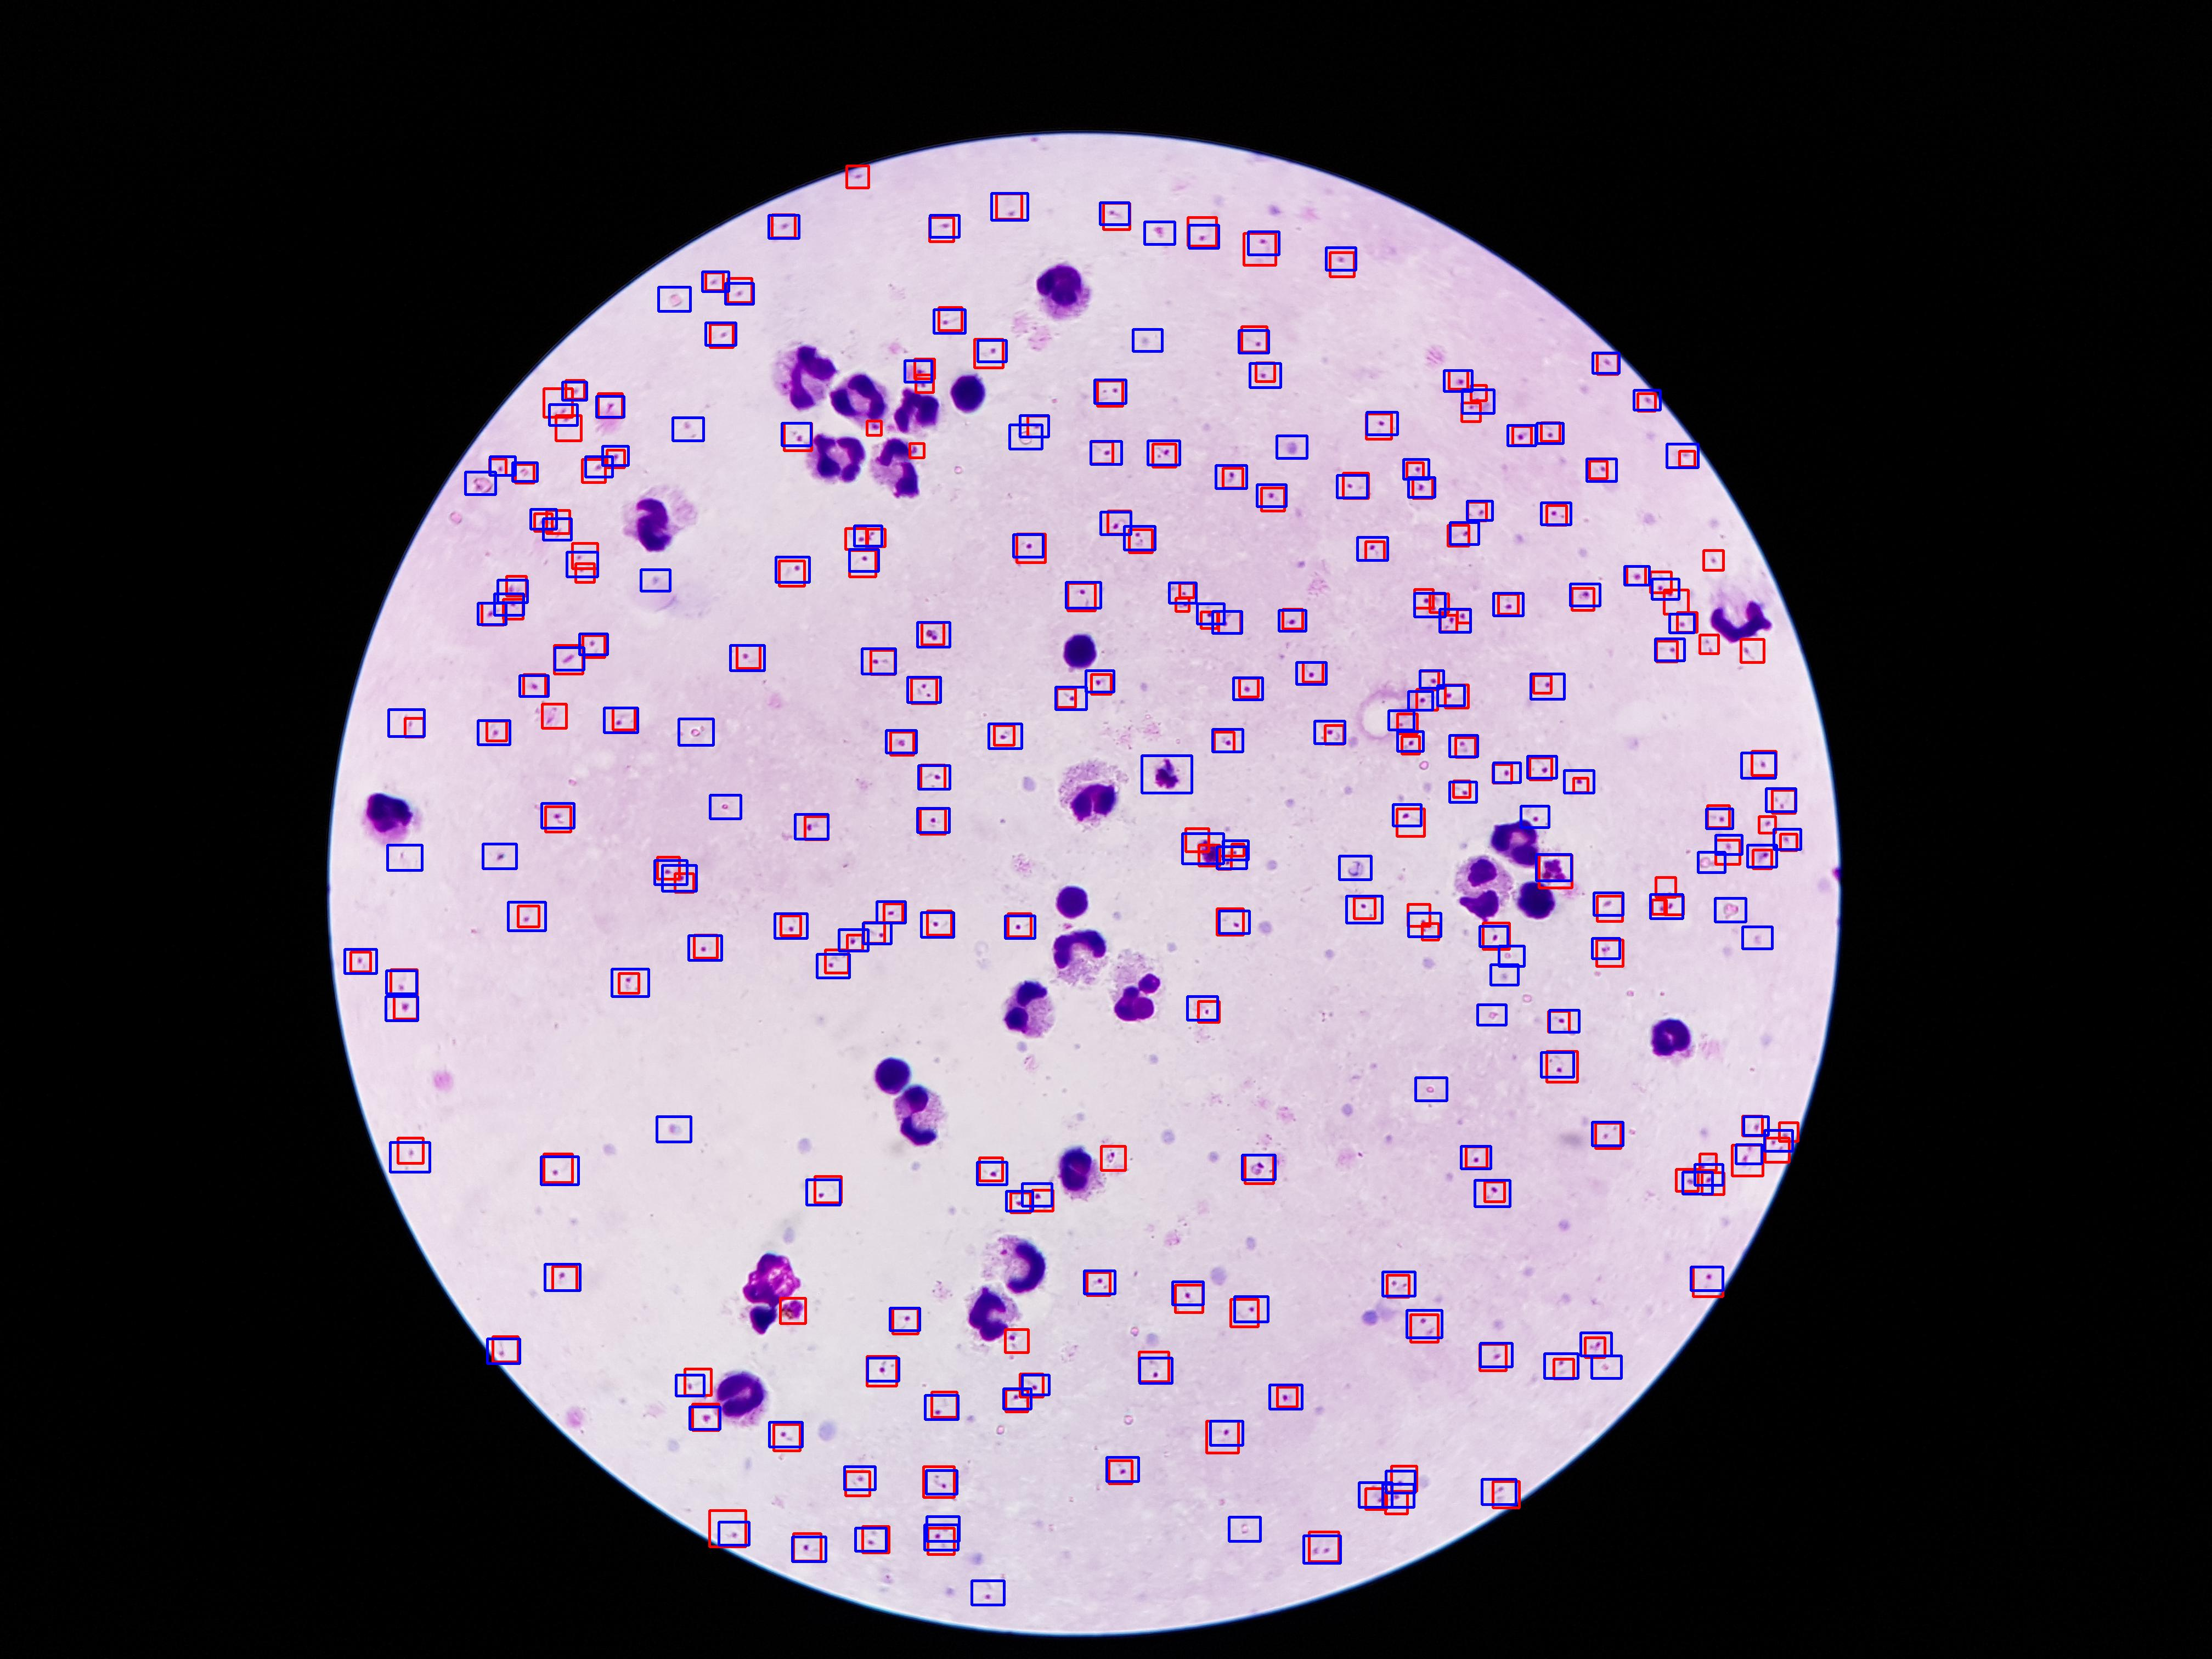
\includegraphics[width=\linewidth]{./img/full-predictions/result5-v7.jpg}
   \caption{Exemplo com muitos protozoários e suas respectivas detecções pela YOLOv7 \emph{X}.} \label{ex:muitos}
 \end{figure}

Apesar dos resultados superiores da YOLOv7 \emph{X} no tocante ao mAP@0.5 se mostrarem melhores que todos os demais modelos avaliados, não é possível afirmar a supremacia dessa solução perante as demais, haja vista, por exemplo, a menor precisão desse modelo frente à YOLOv5 \emph{Small}, a qual possui $\SI{90.09}{\percent}$ menos parâmetros. Seriam necessários mais experimentos e uma análise estatística cuidadosa para derivar conclusões nesse sentido. De maneira geral, todos os modelos mostraram-se competitivos para a tarefa, de natureza realística e com um grau de dificuldade acentuado pela área das caixas delimitadoras e pela distribuição uniforme de sua disposição nas imagens.



